\xiti
\begin{xiaotis}

\xiaoti{下面的说法正确吗?为什么?}
\begin{xiaoxiaotis}

    \xxt{线段 $AB$ 在平面 $\alpha$ 内,直线 $AB$ 不全在平面 $\alpha$ 内;}

    \xxt{平面 $\alpha$ 和 $\beta$ 只有一个公共点。}

\end{xiaoxiaotis}

\xiaoti{为什么有的自行车后轮旁只安装一只撑脚?}

\xiaoti{三角形、梯形是否一定是平面图形?为什么?}

\xiaoti{}%
\begin{xiaoxiaotis}%
    \xxt[\xxtsep]{不共面的四点可以确定几个平面?}

    \xxt{三条直线两两平行,但不共面,它们可以确定几个平面?}

    \xxt{共点的三条直线可以确定几个平面?}

\end{xiaoxiaotis}

\xiaoti{一条直线过平面内一点与平面外一点,它和这个平面有几个公共点?为什么?}


% TODO: wrapfigure 在这里无法正常使用
\begin{minipage}{10cm}
    \jiange
    \xiaoti{一条直线与两条平行直线都相交。证明:这三条直线在同一个平面内。}

    \xiaoti{过已知直线外一点与这条直线上的三点分别画三条直线。证明:这三条直线在同一个平面内。}

    \xiaoti{四条线段顺次首尾连接,所得的图形一定是平面图形吗?为什么?}

    \xiaoti{怎样用两根细绳来检查一张桌子的四条腿的下端,是否在同一个平面内。}

    \xiaoti{画出图中水平放置的四边形 $OABC$ 的直观图。}

    \xiaoti{画水平放置的等腰梯形和平行四边形的直观图。}
\end{minipage}
\quad
\begin{minipage}{5cm}
    \centering
    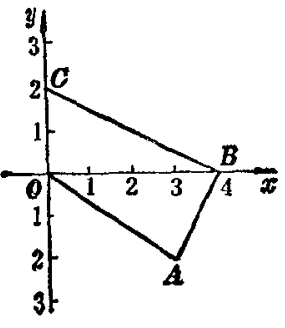
\includegraphics[width=4cm]{../pic/ltjh-ch1-xiti1-10.png}\\
    (第 10 题)
\end{minipage}


\end{xiaotis}

